% ============================================================================
% Chapter 4: Convolutional Neural Networks (CNN)
% ============================================================================
\chapter{Convolutional Neural Networks (CNN)}
\label{ch:cnn}

\noindent\textit{This chapter presents convolutional neural networks, a family of
architectures specialized for processing spatially structured data.
We derive the fundamental operations, study historical and modern
architectures, and mathematically prove the properties that make
residual connections successful.}\medskip

% ----------------------------------------------------------------------------
\section{Motivations}
\label{sec:cnn-motivations}
\index{CNN!motivations}

Fully connected networks have three major limitations for image
processing:

\begin{definition}[Inductive principles of CNNs]
CNNs exploit three principles:
\begin{enumerate}
  \item \textbf{Locality}: visual features are defined by local patterns
    (edges, textures).
    \index{locality}
  \item \textbf{Translation invariance}: a visual pattern can appear
    anywhere in the image.
    \index{translation invariance}
  \item \textbf{Parameter sharing}: the same filter is applied to all
    spatial positions, drastically reducing the number of parameters.
    \index{parameter sharing}
\end{enumerate}
\end{definition}

\begin{remark}[Parameter reduction]
For a $224 \times 224 \times 3$ image, a fully connected layer to 1000
neurons requires $224 \times 224 \times 3 \times 1000 \approx 150$M
parameters. A convolutional layer with 64 filters of size $3 \times 3$
requires only $3 \times 3 \times 3 \times 64 = 1\,728$ parameters.
\end{remark}

% ----------------------------------------------------------------------------
\section{Convolution operation}
\label{sec:convolution}
\index{convolution}

\subsection{2D discrete convolution}

For an input $\mathbf{X} \in \R^{H \times W}$ and a kernel
$\mathbf{K} \in \R^{k_H \times k_W}$, the discrete convolution
(more precisely, cross-correlation) is:

\begin{keyformulas}[title=\textbf{2D Convolution}]
\begin{equation}
(\mathbf{X} * \mathbf{K})[i, j] = \sum_{m=0}^{k_H - 1} \sum_{n=0}^{k_W - 1}
  \mathbf{X}[i + m, j + n] \cdot \mathbf{K}[m, n]
\label{eq:conv2d}
\end{equation}
\end{keyformulas}

\subsection{Output size}

\begin{theorem}[Output size formula]
For an input of size $H \times W$, a kernel $k \times k$, padding
$p$, and stride $s$, the output size is:
\begin{equation}
H_{\text{out}} = \left\lfloor \frac{H - k + 2p}{s} \right\rfloor + 1, \qquad
W_{\text{out}} = \left\lfloor \frac{W - k + 2p}{s} \right\rfloor + 1
\label{eq:conv-output-size}
\end{equation}
\end{theorem}

\begin{example}[Size calculation]
Input $32 \times 32$, kernel $5 \times 5$, padding $p = 2$, stride $s = 1$:
\[
H_{\text{out}} = \left\lfloor \frac{32 - 5 + 4}{1} \right\rfloor + 1 = 32
\]
Padding $p = \lfloor k/2 \rfloor$ preserves the spatial size
(``same padding'').
\end{example}

\subsection{Multi-channel convolution}

For $C_{\text{in}}$ input channels and $C_{\text{out}}$ filters:
\begin{equation}
\mathbf{Y}[c_{\text{out}}, i, j] = b_{c_{\text{out}}} +
\sum_{c_{\text{in}}=0}^{C_{\text{in}}-1}
\sum_{m=0}^{k_H-1} \sum_{n=0}^{k_W-1}
\mathbf{X}[c_{\text{in}}, i{+}m, j{+}n] \cdot
\mathbf{K}[c_{\text{out}}, c_{\text{in}}, m, n]
\end{equation}

Total number of parameters: $C_{\text{out}} \times (C_{\text{in}} \times k_H \times k_W + 1)$.

\subsection{Convolution operation diagram}

\begin{center}
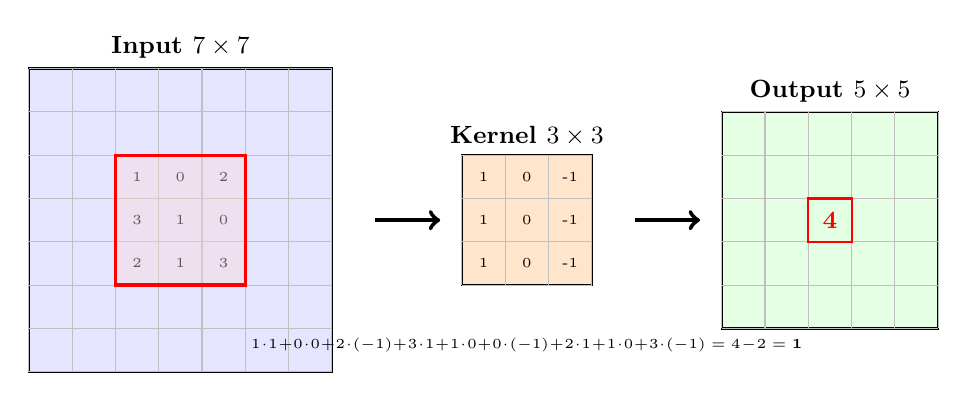
\begin{tikzpicture}[scale=0.55]
  % Input
  \draw[fill=blue!10, thick] (0,0) rectangle (7,7);
  \node[above, font=\small\bfseries] at (3.5, 7) {Input $7 \times 7$};

  % Grid
  \foreach \i in {0,...,7} {
    \draw[gray!50] (\i, 0) -- (\i, 7);
    \draw[gray!50] (0, \i) -- (7, \i);
  }

  % Values in the input (sub-region)
  \foreach \i/\j/\v in {
    2/4/1, 3/4/0, 4/4/2,
    2/3/3, 3/3/1, 4/3/0,
    2/2/2, 3/2/1, 4/2/3} {
    \node[font=\tiny] at (\i+0.5, \j+0.5) {\v};
  }

  % Receptive field highlight
  \draw[red, very thick, fill=red!15, fill opacity=0.4] (2,2) rectangle (5,5);

  % Arrow
  \draw[->, ultra thick] (8, 3.5) -- (9.5, 3.5);

  % Kernel
  \draw[fill=orange!20, thick] (10, 2) rectangle (13, 5);
  \foreach \i in {10,...,13} {
    \draw[gray!50] (\i, 2) -- (\i, 5);
    \draw[gray!50] (10, \i-8) -- (13, \i-8);
  }
  \foreach \i/\j/\v in {
    10/4/1, 11/4/0, 12/4/-1,
    10/3/1, 11/3/0, 12/3/-1,
    10/2/1, 11/2/0, 12/2/-1} {
    \node[font=\tiny] at (\i+0.5, \j+0.5) {\v};
  }
  \node[above, font=\small\bfseries] at (11.5, 5) {Kernel $3 \times 3$};

  % Arrow
  \draw[->, ultra thick] (14, 3.5) -- (15.5, 3.5);

  % Output
  \draw[fill=green!10, thick] (16, 1) rectangle (21, 6);
  \foreach \i in {16,...,21} {
    \draw[gray!50] (\i, 1) -- (\i, 6);
  }
  \foreach \i in {1,...,6} {
    \draw[gray!50] (16, \i) -- (21, \i);
  }

  % Computed value
  \node[font=\small, red] at (18.5, 3.5) {$\mathbf{4}$};
  \draw[red, thick] (18, 3) rectangle (19, 4);

  \node[above, font=\small\bfseries] at (18.5, 6) {Output $5 \times 5$};

  % Computation
  \node[below, font=\tiny, text width=7cm, align=center] at (11.5, 1) {
    $1 \cdot 1 + 0 \cdot 0 + 2 \cdot (-1) + 3 \cdot 1 + 1 \cdot 0 + 0 \cdot (-1)
     + 2 \cdot 1 + 1 \cdot 0 + 3 \cdot (-1) = 4 - 2 = \mathbf{1}$
  };
\end{tikzpicture}
\end{center}

% ----------------------------------------------------------------------------
\section{Pooling layers}
\label{sec:pooling}
\index{pooling}

\begin{keyformulas}[title=\textbf{Pooling operations}]
For a pooling window of size $k \times k$:
\begin{align}
\text{Max Pooling:} \quad y[i,j] &= \max_{0 \leq m,n < k} x[i \cdot s + m,\; j \cdot s + n]
\label{eq:maxpool} \\
\text{Average Pooling:} \quad y[i,j] &= \frac{1}{k^2} \sum_{m=0}^{k-1} \sum_{n=0}^{k-1}
  x[i \cdot s + m,\; j \cdot s + n]
\label{eq:avgpool}
\end{align}
\end{keyformulas}

\begin{definition}[Global Average Pooling (GAP)]
\index{Global Average Pooling}
GAP computes the average over the entire feature map:
\begin{equation}
\text{GAP}(\mathbf{X})[c] = \frac{1}{H \times W} \sum_{i=1}^{H} \sum_{j=1}^{W}
  \mathbf{X}[c, i, j]
\end{equation}
It replaces final fully connected layers in modern architectures,
reducing the number of parameters and overfitting.
\end{definition}

% ----------------------------------------------------------------------------
\section{Classical architectures}
\label{sec:classic-archs}

\subsection{LeNet-5 (1998)}
\index{LeNet-5}

\begin{center}
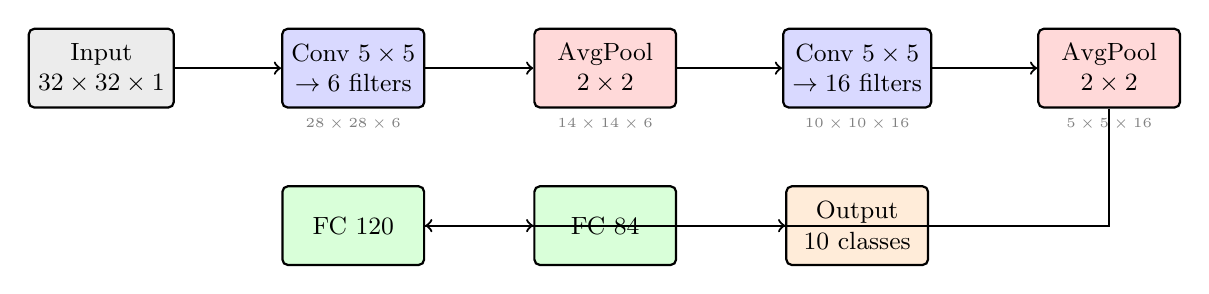
\begin{tikzpicture}[
  block/.style={rectangle, draw, thick, fill=#1, minimum height=1cm,
                minimum width=1.8cm, font=\small, align=center, rounded corners=2pt},
  block/.default={blue!15},
  arr/.style={->, thick}
]
  \node[block=gray!15] (input) at (0,0) {Input\\$32 \times 32 \times 1$};
  \node[block] (c1) at (3.2,0) {Conv $5 \times 5$\\$\to 6$ filters};
  \node[block=red!15] (p1) at (6.4,0) {AvgPool\\$2 \times 2$};
  \node[block] (c2) at (9.6,0) {Conv $5 \times 5$\\$\to 16$ filters};
  \node[block=red!15] (p2) at (12.8,0) {AvgPool\\$2 \times 2$};
  \node[block=green!15] (fc1) at (3.2,-2) {FC 120};
  \node[block=green!15] (fc2) at (6.4,-2) {FC 84};
  \node[block=orange!15] (out) at (9.6,-2) {Output\\10 classes};

  \draw[arr] (input) -- (c1);
  \draw[arr] (c1) -- (p1);
  \draw[arr] (p1) -- (c2);
  \draw[arr] (c2) -- (p2);
  \draw[arr] (p2) |- (fc1);
  \draw[arr] (fc1) -- (fc2);
  \draw[arr] (fc2) -- (out);

  % Sizes
  \node[below, font=\tiny, gray] at (c1.south) {$28 \times 28 \times 6$};
  \node[below, font=\tiny, gray] at (p1.south) {$14 \times 14 \times 6$};
  \node[below, font=\tiny, gray] at (c2.south) {$10 \times 10 \times 16$};
  \node[below, font=\tiny, gray] at (p2.south) {$5 \times 5 \times 16$};
\end{tikzpicture}
\end{center}

\subsection{AlexNet (2012)}
\index{AlexNet}

AlexNet \cite{krizhevsky2012imagenet} marked the return of neural networks
in computer vision, winning the ImageNet 2012 challenge with a top-5
error of 15.3\% (compared to 26.2\% for classical methods). Key
innovations: ReLU, Dropout (cf.\ Chapter~\ref{ch:regularization}),
GPU training.

\subsection{VGGNet (2014)}
\index{VGGNet}

VGGNet \cite{simonyan2015very} demonstrated the importance of depth
with a homogeneous architecture using only $3 \times 3$ convolutions.

\begin{remark}[Receptive field of stacked convolutions]
Two stacked $3 \times 3$ convolutions have a receptive field of $5 \times 5$,
and three $3 \times 3$ convolutions have a receptive field of $7 \times 7$, but with
fewer parameters: $3 \times (3^2 C^2) = 27C^2$ vs $7^2 C^2 = 49C^2$.
\end{remark}

\subsection{ResNet (2015)}
\label{sec:resnet}
\index{ResNet}

\subsubsection{Residual connection}

\begin{keyformulas}[title=\textbf{Residual block}]
\begin{equation}
\mathbf{y} = \mathcal{F}(\mathbf{x}, \{W_i\}) + \mathbf{x}
\label{eq:residual-block}
\end{equation}
where $\mathcal{F}(\mathbf{x}, \{W_i\})$ represents the residual
transformation (typically Conv-BN-ReLU-Conv-BN).
\end{keyformulas}

\begin{center}
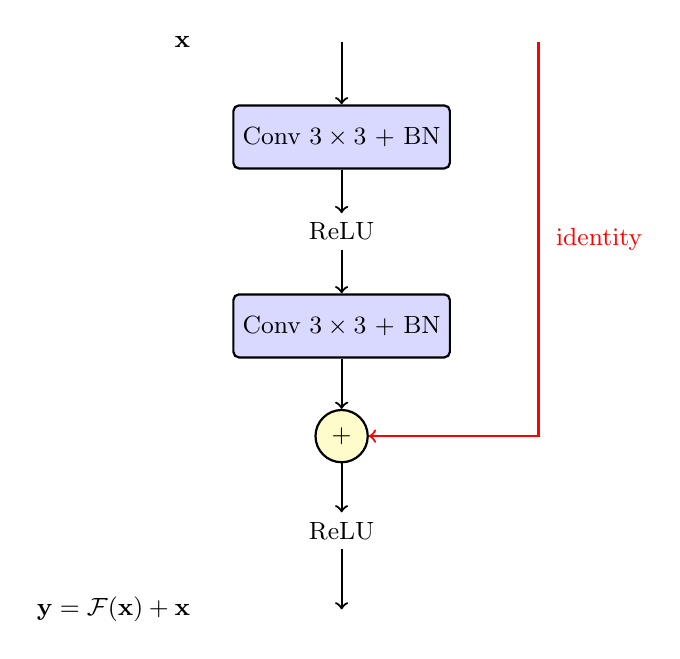
\begin{tikzpicture}[
  block/.style={rectangle, draw, thick, fill=blue!15, minimum height=0.8cm,
                minimum width=2.5cm, font=\small, rounded corners=2pt},
  arr/.style={->, thick},
  plus/.style={circle, draw, thick, fill=yellow!20, minimum size=6mm,
               font=\small}
]
  \node[block] (conv1) at (0, 0) {Conv $3 \times 3$ + BN};
  \node[font=\small] (relu1) at (0, -1.2) {ReLU};
  \node[block] (conv2) at (0, -2.4) {Conv $3 \times 3$ + BN};
  \node[plus] (add) at (0, -3.8) {$+$};
  \node[font=\small] (relu2) at (0, -5.0) {ReLU};

  % Main connection
  \draw[arr] (0, 1.2) -- (conv1);
  \draw[arr] (conv1) -- (relu1);
  \draw[arr] (relu1) -- (conv2);
  \draw[arr] (conv2) -- (add);
  \draw[arr] (add) -- (relu2);
  \draw[arr] (relu2) -- (0, -6.0);

  % Skip connection
  \draw[arr, red, thick] (2.5, 1.2) -- (2.5, -3.8) -- (add);
  \node[red, font=\small, right] at (2.6, -1.3) {identity};

  % Labels
  \node[left, font=\small] at (-1.8, 1.2) {$\mathbf{x}$};
  \node[left, font=\small] at (-1.8, -6.0) {$\mathbf{y} = \mathcal{F}(\mathbf{x}) + \mathbf{x}$};
\end{tikzpicture}
\end{center}

\subsubsection{Proof of gradient flow preservation}

\begin{theorem}[Gradient flow in ResNet]
\label{thm:resnet-gradient}
Consider a network of $L$ residual blocks. The output of block $l$ is
$\mathbf{x}_{l+1} = \mathcal{F}_l(\mathbf{x}_l) + \mathbf{x}_l$. Then
the output of block $L$ can be expressed as:
\begin{equation}
\mathbf{x}_L = \mathbf{x}_l + \sum_{i=l}^{L-1} \mathcal{F}_i(\mathbf{x}_i)
\label{eq:resnet-unrolled}
\end{equation}

The gradient of the loss $\mathcal{L}$ with respect to $\mathbf{x}_l$ is:
\begin{align}
\frac{\partial \mathcal{L}}{\partial \mathbf{x}_l}
&= \frac{\partial \mathcal{L}}{\partial \mathbf{x}_L}
   \cdot \frac{\partial \mathbf{x}_L}{\partial \mathbf{x}_l} \nonumber \\
&= \frac{\partial \mathcal{L}}{\partial \mathbf{x}_L}
   \left(1 + \frac{\partial}{\partial \mathbf{x}_l}
   \sum_{i=l}^{L-1} \mathcal{F}_i(\mathbf{x}_i)\right)
\label{eq:resnet-gradient}
\end{align}

\textbf{Proof.}
By recurrence, $\mathbf{x}_{l+1} = \mathcal{F}_l(\mathbf{x}_l) + \mathbf{x}_l$
and $\mathbf{x}_{l+2} = \mathcal{F}_{l+1}(\mathbf{x}_{l+1}) + \mathbf{x}_{l+1}
= \mathcal{F}_{l+1}(\mathbf{x}_{l+1}) + \mathcal{F}_l(\mathbf{x}_l) + \mathbf{x}_l$.
By induction, we obtain (\ref{eq:resnet-unrolled}). Differentiating and
applying the chain rule, the $\mathbf{1}$ term in
(\ref{eq:resnet-gradient}) guarantees that the gradient never vanishes
completely, even if $\frac{\partial \mathcal{F}_i}{\partial \mathbf{x}_l}
\to 0$.
\end{theorem}

\begin{intuition}[title=\textbf{Why ResNet works}]
The ``$+1$'' term in Equation~(\ref{eq:resnet-gradient}) creates a
``gradient highway'' that bypasses the nonlinear layers. The network
only needs to learn the \textbf{residual}
$\mathcal{F}(\mathbf{x}) = \mathbf{y} - \mathbf{x}$, which is often close
to zero and therefore easier to learn.
\end{intuition}

% ----------------------------------------------------------------------------
\section{Transfer learning and fine-tuning}
\label{sec:transfer-learning}
\index{transfer learning}\index{fine-tuning}

\begin{definition}[Transfer learning]
Transfer learning consists of reusing a model pre-trained on a large
dataset (e.g.\ ImageNet) for a new task, potentially with a smaller
dataset.
\end{definition}

Common strategies:
\begin{enumerate}
  \item \textbf{Feature extractor}: freeze all convolutional layers and
    only train the final classifier.
  \item \textbf{Partial fine-tuning}: unfreeze the last convolutional
    layers with a reduced learning rate.
  \item \textbf{Full fine-tuning}: train the entire network with a low
    learning rate.
\end{enumerate}

\begin{bestpractice}[title=\textbf{Learning rate for fine-tuning}]
Use a learning rate 10 to 100 times smaller than for initial training.
Regularization techniques (Chapter~\ref{ch:regularization}) are crucial
to avoid overfitting during fine-tuning.
\end{bestpractice}

% ----------------------------------------------------------------------------
\section{PyTorch implementation}
\label{sec:cnn-pytorch}

\begin{codeblock}[title=\textbf{CNN for CIFAR-10 with full training}]
\begin{minted}{python}
import torch
import torch.nn as nn
import torch.optim as optim
from torchvision import datasets, transforms
from torch.utils.data import DataLoader

# --- CNN Architecture ---
class CIFAR10Net(nn.Module):
    def __init__(self, num_classes=10):
        super().__init__()
        self.features = nn.Sequential(
            # Block 1: 32x32x3 -> 32x32x64 -> 16x16x64
            nn.Conv2d(3, 64, kernel_size=3, padding=1),
            nn.BatchNorm2d(64),
            nn.ReLU(inplace=True),
            nn.Conv2d(64, 64, kernel_size=3, padding=1),
            nn.BatchNorm2d(64),
            nn.ReLU(inplace=True),
            nn.MaxPool2d(2, 2),
            nn.Dropout2d(0.25),

            # Block 2: 16x16x64 -> 16x16x128 -> 8x8x128
            nn.Conv2d(64, 128, kernel_size=3, padding=1),
            nn.BatchNorm2d(128),
            nn.ReLU(inplace=True),
            nn.Conv2d(128, 128, kernel_size=3, padding=1),
            nn.BatchNorm2d(128),
            nn.ReLU(inplace=True),
            nn.MaxPool2d(2, 2),
            nn.Dropout2d(0.25),

            # Block 3: 8x8x128 -> 8x8x256 -> 4x4x256
            nn.Conv2d(128, 256, kernel_size=3, padding=1),
            nn.BatchNorm2d(256),
            nn.ReLU(inplace=True),
            nn.Conv2d(256, 256, kernel_size=3, padding=1),
            nn.BatchNorm2d(256),
            nn.ReLU(inplace=True),
            nn.MaxPool2d(2, 2),
            nn.Dropout2d(0.25),
        )
        self.classifier = nn.Sequential(
            nn.AdaptiveAvgPool2d(1),   # Global Average Pooling
            nn.Flatten(),
            nn.Linear(256, 128),
            nn.ReLU(inplace=True),
            nn.Dropout(0.5),
            nn.Linear(128, num_classes)
        )

    def forward(self, x):
        x = self.features(x)
        x = self.classifier(x)
        return x

# --- Data preparation ---
transform_train = transforms.Compose([
    transforms.RandomCrop(32, padding=4),
    transforms.RandomHorizontalFlip(),
    transforms.ColorJitter(brightness=0.2, contrast=0.2),
    transforms.ToTensor(),
    transforms.Normalize((0.4914, 0.4822, 0.4465),
                         (0.2470, 0.2435, 0.2616))
])

transform_test = transforms.Compose([
    transforms.ToTensor(),
    transforms.Normalize((0.4914, 0.4822, 0.4465),
                         (0.2470, 0.2435, 0.2616))
])

train_set = datasets.CIFAR10('./data', train=True,
                             download=True, transform=transform_train)
test_set = datasets.CIFAR10('./data', train=False,
                            transform=transform_test)
train_loader = DataLoader(train_set, batch_size=128,
                          shuffle=True, num_workers=2)
test_loader = DataLoader(test_set, batch_size=256,
                         shuffle=False, num_workers=2)

# --- Training ---
device = torch.device('cuda' if torch.cuda.is_available() else 'cpu')
model = CIFAR10Net().to(device)
criterion = nn.CrossEntropyLoss()
optimizer = optim.AdamW(model.parameters(), lr=1e-3, weight_decay=1e-4)
scheduler = optim.lr_scheduler.CosineAnnealingLR(optimizer, T_max=100)

print(f"Parameters: {sum(p.numel() for p in model.parameters()):,}")

for epoch in range(100):
    # Training
    model.train()
    train_loss, correct, total = 0.0, 0, 0
    for inputs, targets in train_loader:
        inputs, targets = inputs.to(device), targets.to(device)
        optimizer.zero_grad()
        outputs = model(inputs)
        loss = criterion(outputs, targets)
        loss.backward()
        optimizer.step()
        train_loss += loss.item() * inputs.size(0)
        correct += (outputs.argmax(1) == targets).sum().item()
        total += targets.size(0)

    # Evaluation
    model.eval()
    test_correct, test_total = 0, 0
    with torch.no_grad():
        for inputs, targets in test_loader:
            inputs, targets = inputs.to(device), targets.to(device)
            outputs = model(inputs)
            test_correct += (outputs.argmax(1) == targets).sum().item()
            test_total += targets.size(0)

    scheduler.step()
    if (epoch + 1) % 10 == 0:
        print(f"Epoch {epoch+1:3d} | "
              f"Train Loss: {train_loss/total:.4f} | "
              f"Train Acc: {correct/total:.4f} | "
              f"Test Acc: {test_correct/test_total:.4f}")
\end{minted}
\end{codeblock}

\begin{codeoutput}
\begin{verbatim}
Parameters: 952,202
Epoch  10 | Train Loss: 0.8234 | Train Acc: 0.7142 | Test Acc: 0.7856
Epoch  20 | Train Loss: 0.5321 | Train Acc: 0.8134 | Test Acc: 0.8523
Epoch  30 | Train Loss: 0.4012 | Train Acc: 0.8612 | Test Acc: 0.8802
Epoch  40 | Train Loss: 0.3245 | Train Acc: 0.8876 | Test Acc: 0.8945
Epoch  50 | Train Loss: 0.2678 | Train Acc: 0.9056 | Test Acc: 0.9034
Epoch  60 | Train Loss: 0.2234 | Train Acc: 0.9213 | Test Acc: 0.9098
Epoch  70 | Train Loss: 0.1878 | Train Acc: 0.9345 | Test Acc: 0.9145
Epoch  80 | Train Loss: 0.1534 | Train Acc: 0.9467 | Test Acc: 0.9178
Epoch  90 | Train Loss: 0.1312 | Train Acc: 0.9534 | Test Acc: 0.9201
Epoch 100 | Train Loss: 0.1198 | Train Acc: 0.9578 | Test Acc: 0.9218
\end{verbatim}
\end{codeoutput}

% ----------------------------------------------------------------------------
\section{Transfer learning with a pre-trained model}
\label{sec:transfer-code}

\begin{codeblock}[title=\textbf{Fine-tuning a pre-trained ResNet-18}]
\begin{minted}{python}
import torchvision.models as models

# Load ResNet-18 pre-trained on ImageNet
model = models.resnet18(weights=models.ResNet18_Weights.DEFAULT)

# Freeze convolutional layers
for param in model.parameters():
    param.requires_grad = False

# Replace the last FC layer
num_features = model.fc.in_features
model.fc = nn.Sequential(
    nn.Dropout(0.3),
    nn.Linear(num_features, 10)
)
model = model.to(device)

# Only the last layer is trained
optimizer = optim.Adam(model.fc.parameters(), lr=1e-3)

# Phase 2: unfreeze the last 2 blocks for fine-tuning
for param in model.layer3.parameters():
    param.requires_grad = True
for param in model.layer4.parameters():
    param.requires_grad = True

optimizer = optim.AdamW([
    {'params': model.layer3.parameters(), 'lr': 1e-5},
    {'params': model.layer4.parameters(), 'lr': 1e-4},
    {'params': model.fc.parameters(), 'lr': 1e-3},
], weight_decay=1e-4)
\end{minted}
\end{codeblock}

% ----------------------------------------------------------------------------
\section{Ablation study}
\label{sec:cnn-ablation}

\begin{codeblock}[title=\textbf{Ablation: kernel size, number of filters, depth}]
\begin{minted}{python}
import pandas as pd

def build_cnn(kernel_size, num_filters, num_blocks):
    """Build a parameterizable CNN for ablation."""
    layers = []
    in_channels = 3
    for i in range(num_blocks):
        out_channels = num_filters * (2 ** min(i, 2))
        pad = kernel_size // 2
        layers.extend([
            nn.Conv2d(in_channels, out_channels, kernel_size, padding=pad),
            nn.BatchNorm2d(out_channels),
            nn.ReLU(inplace=True),
            nn.MaxPool2d(2, 2),
        ])
        in_channels = out_channels
    layers.extend([nn.AdaptiveAvgPool2d(1), nn.Flatten(),
                   nn.Linear(in_channels, 10)])
    return nn.Sequential(*layers)

configs = [
    {'kernel_size': 3, 'num_filters': 32, 'num_blocks': 3},
    {'kernel_size': 5, 'num_filters': 32, 'num_blocks': 3},
    {'kernel_size': 3, 'num_filters': 64, 'num_blocks': 3},
    {'kernel_size': 3, 'num_filters': 32, 'num_blocks': 5},
]

results = []
for cfg in configs:
    model = build_cnn(**cfg).to(device)
    n_params = sum(p.numel() for p in model.parameters())
    # Train for 30 epochs (simplified)
    optimizer = optim.AdamW(model.parameters(), lr=1e-3)
    best_acc = 0.0
    for epoch in range(30):
        model.train()
        for x, y in train_loader:
            x, y = x.to(device), y.to(device)
            optimizer.zero_grad()
            loss = criterion(model(x), y)
            loss.backward()
            optimizer.step()
        model.eval()
        correct = sum((model(x.to(device)).argmax(1) == y.to(device)).sum().item()
                      for x, y in test_loader)
        best_acc = max(best_acc, correct / len(test_set))
    results.append({**cfg, 'params': n_params, 'accuracy': best_acc})

print(pd.DataFrame(results).to_string(index=False))
\end{minted}
\end{codeblock}

\begin{codeoutput}
\begin{verbatim}
 kernel_size  num_filters  num_blocks  params   accuracy
           3           32           3   52778     0.8734
           5           32           3  143642     0.8812
           3           64           3  207946     0.9015
           3           32           5  218410     0.8956
\end{verbatim}
\end{codeoutput}

\begin{remark}[Ablation observations]
\begin{itemize}
  \item Doubling the number of filters ($32 \to 64$) improves performance
    more than increasing kernel size or depth.
  \item $5 \times 5$ kernels provide a marginal gain over $3 \times 3$
    for a significant parameter cost.
  \item Depth helps, but with diminishing returns without residual
    connections.
\end{itemize}
\end{remark}

% ----------------------------------------------------------------------------
\section{Depthwise separable convolutions}
\label{sec:depthwise-separable}
\index{convolution!depthwise separable}

\begin{keyformulas}[title=\textbf{Depthwise separable convolution}]
A standard convolution $C_{\text{in}} \to C_{\text{out}}$ with kernel $k \times k$
costs $C_{\text{in}} \cdot C_{\text{out}} \cdot k^2$ multiplications per position.
The separable convolution decomposes into:
\begin{enumerate}
  \item \textbf{Depthwise}: one $k \times k$ filter per channel, cost $C_{\text{in}} \cdot k^2$
  \item \textbf{Pointwise}: $1 \times 1$ convolution to combine, cost $C_{\text{in}} \cdot C_{\text{out}}$
\end{enumerate}
Reduction ratio:
\begin{equation}
\frac{C_{\text{in}} \cdot k^2 + C_{\text{in}} \cdot C_{\text{out}}}{C_{\text{in}} \cdot C_{\text{out}} \cdot k^2}
= \frac{1}{C_{\text{out}}} + \frac{1}{k^2}
\end{equation}
For $C_{\text{out}} = 256$ and $k = 3$: reduction by a factor of $\approx 8\text{--}9\times$.
\end{keyformulas}

% ----------------------------------------------------------------------------
\section{State-of-the-art techniques}
\label{sec:cnn-sota}

\begin{sota}[title=\textbf{Modern CNN architectures}]
\begin{description}
  \item[EfficientNet] \cite{tan2019efficientnet}: balanced compound scaling
    in depth, width, and resolution:
    \begin{equation}
      d = \alpha^\phi, \quad w = \beta^\phi, \quad r = \gamma^\phi
      \quad \text{subject to} \quad \alpha \cdot \beta^2 \cdot \gamma^2 \approx 2
    \end{equation}
    \index{EfficientNet}

  \item[ConvNeXt] \cite{liu2022convnet}: modernization of ResNet with
    elements borrowed from Transformers (cf.\ Chapter~\ref{ch:attention}):
    $7 \times 7$ depthwise kernels, LayerNorm, GELU, fewer activation functions.
    Achieves performance comparable to Vision Transformers.
    \index{ConvNeXt}

  \item[Deformable convolutions] \cite{dai2017deformable}: learn spatial
    offsets to adapt the receptive field shape:
    \begin{equation}
      y(\mathbf{p}_0) = \sum_{n=1}^{N} w_n \cdot x(\mathbf{p}_0 + \mathbf{p}_n + \Delta\mathbf{p}_n)
    \end{equation}
    where $\Delta\mathbf{p}_n$ are learned offsets.
    \index{convolution!deformable}
\end{description}
\end{sota}

% ----------------------------------------------------------------------------
\section{Exercises}
\label{sec:cnn-exercises}

\begin{exercise}[Dimension calculations \hfill $\bigstar$]
A network receives $128 \times 128 \times 3$ images and successively
applies:
\begin{enumerate}
  \item Conv2d(3, 32, kernel\_size=5, padding=2, stride=1)
  \item MaxPool2d(2, 2)
  \item Conv2d(32, 64, kernel\_size=3, padding=0, stride=2)
  \item Conv2d(64, 128, kernel\_size=3, padding=1, stride=1)
  \item AdaptiveAvgPool2d(1)
\end{enumerate}
Compute the output size and the number of parameters at each layer.
\end{exercise}

\begin{exercise}[Residual block implementation \hfill $\bigstar\bigstar$]
\begin{enumerate}
  \item Implement a complete residual block (with projection when
    dimensions change) in PyTorch.
  \item Build a mini-ResNet (8 layers) for CIFAR-10.
  \item Compare convergence with and without residual connections.
  \item Plot the gradients in the first layers for both cases.
\end{enumerate}
\end{exercise}

\begin{exercise}[Filter visualization \hfill $\bigstar\bigstar$]
\begin{enumerate}
  \item Train a CNN on CIFAR-10 and visualize the filters of the first
    convolutional layer.
  \item Use intermediate \textit{feature maps} to understand what each
    layer detects.
  \item Implement the \textit{Grad-CAM} technique to visualize the image
    regions contributing to the decision.
\end{enumerate}
\end{exercise}

\begin{exercise}[Depthwise separable convolutions \hfill $\bigstar\bigstar$]
\begin{enumerate}
  \item Implement a depthwise separable convolution layer
    (\texttt{nn.Conv2d} with \texttt{groups=in\_channels} + $1 \times 1$ conv).
  \item Replace all $3 \times 3$ convolutions in the CIFAR-10 CNN with
    separable convolutions. Compare the number of parameters and
    accuracy.
  \item Measure the inference time of both versions.
\end{enumerate}
\end{exercise}

\begin{exercise}[Receptive field proof \hfill $\bigstar\bigstar\bigstar$]
\begin{enumerate}
  \item Prove by induction that $n$ stacked $k \times k$ convolutional
    layers with stride $s = 1$ produce a receptive field of size
    $n(k - 1) + 1$.
  \item Generalize for arbitrary strides and dilations.
  \item Compute the effective receptive field of a ResNet-50 and compare
    with the input image size.
  \item Discuss the relationship between receptive field and modeling
    capacity.
\end{enumerate}
\end{exercise}
